\documentclass{article}
\usepackage{amsmath,amsfonts}
\usepackage{graphicx}
\usepackage[margin=1.0in,letterpaper]{geometry}
\usepackage{float}
\usepackage{hyperref}
%\usepackage{subfigure}

% are used to denote commments, everything after it on this line is a comment and while not be processed 

\begin{document}

\title{Orion-Eridanus Superbubble Imaging}
\author{Leonardo Sattler Cassara, e-mail:leosattler@berkeley.edu}
\date{May 6, 2014}
\maketitle

\begin{abstract}

In this lab we work with the $3.6 \ m$ dish from Leuschner Observatory,
measuring the $21 \ cm$ line emissions
from atomic hydrogen (HI), an abundant element in our galaxy. Analysing
features of this line, 
we create an image of the Orion-Eridanus Superbubble, by using the total
flux from HI lines to measure the thickness of a Hydrogen column, and
evidenciating the
bubble shell from the center to the edges. 
The methods for tracking, recording and treating the data
are presented and the choices justified. The final result is the image
of Fig.?, made with $\approx 500$ points, mapping the sky from galactic
latitude $-60^{\circ} $ 
to $-10^{\circ} $ ($b = -10^{\circ}  \rightarrow -70^{\circ}$ (JD)), 
and galactig longitude from $160 ^{\circ} $ 
to $220  ^{\circ}$ ($l = 160  ^{\circ} \rightarrow 220 ^{\circ}$ (JD)).

\end{abstract}

\section{Introduction}

In Radioastronomy, one of the greatest advantages is the hability of
radio antennas on observing the hyperfine energy 
transition of neutral Hydrogen (HI), known as the $21
\ cm$ line, or $1420.4 \ MHz$. This feature is largelly explored due to the fact that this
element is present in the whole universe, and many structuers are comprised of molecular hydrogen.
We explore this fact using the Leuschner dish (Fig.1) to measure the spectra of 
a large scale structure, and identify the HI lines to obtain a direct
measurement of the quantity of this element. 

\begin{figure}[H]
\center
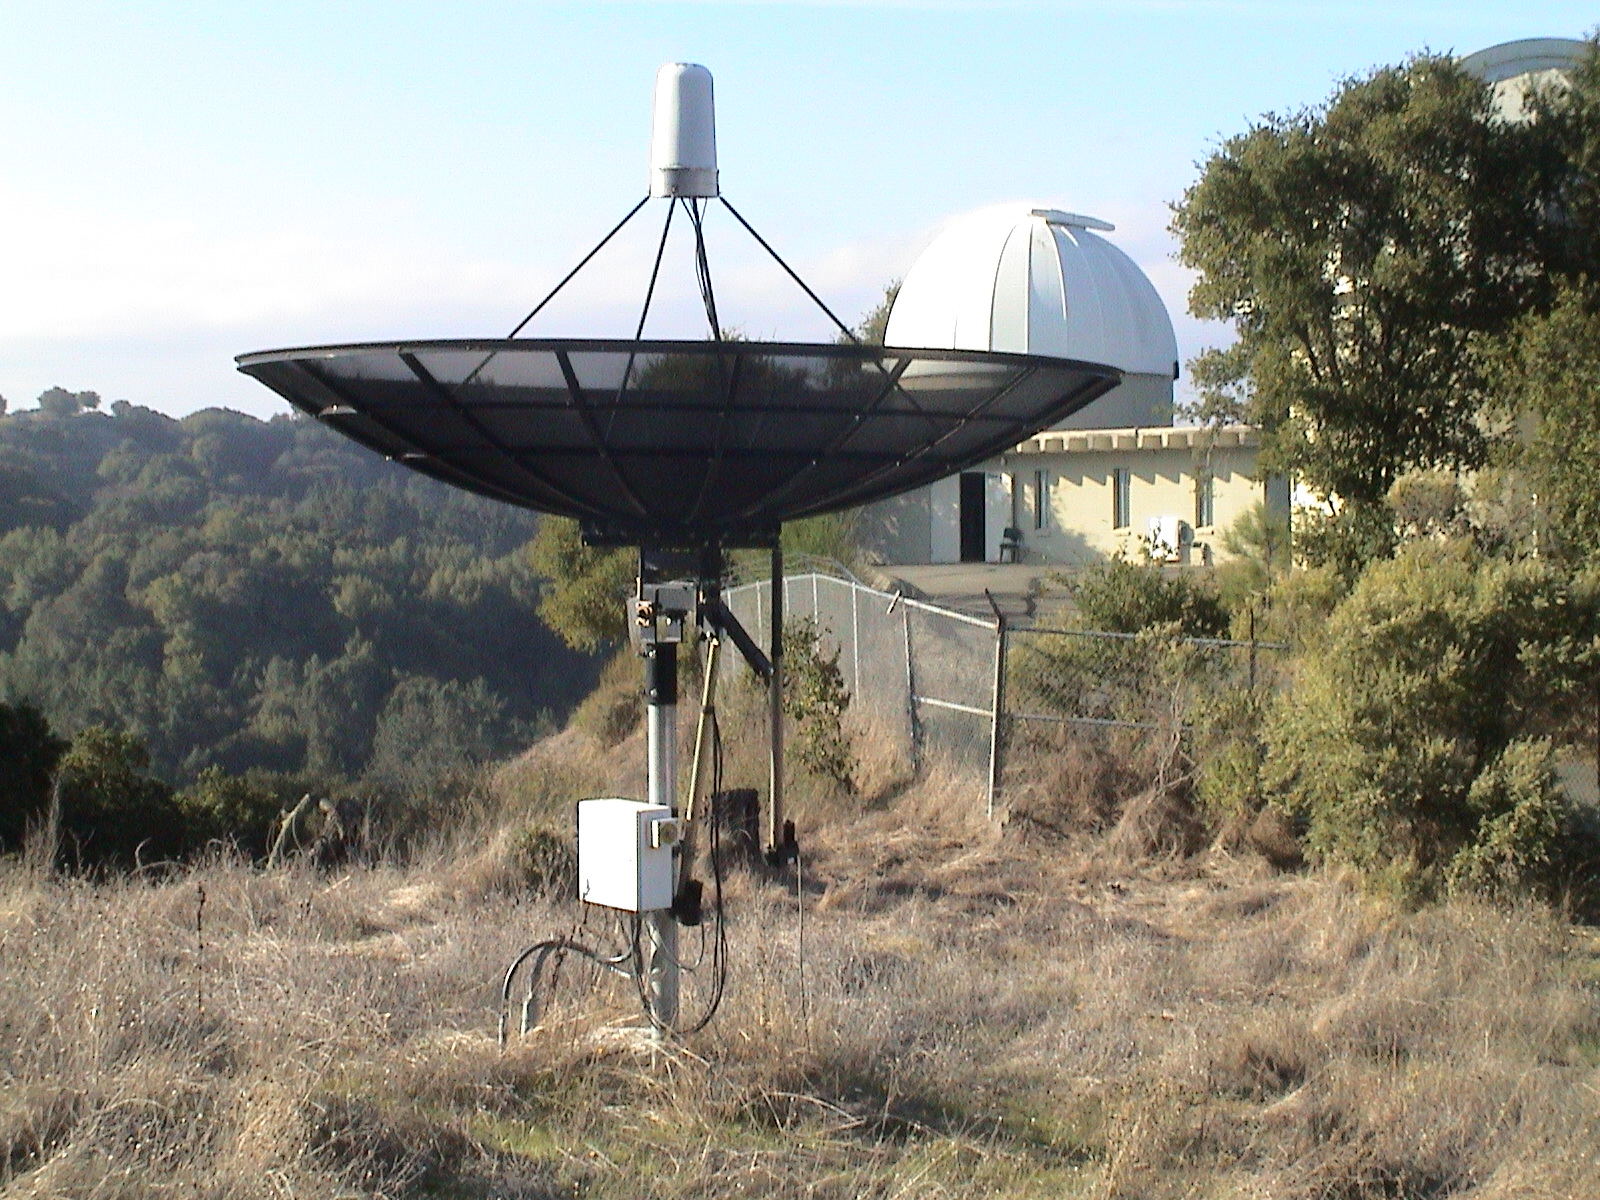
\includegraphics[scale=0.2]{dish.jpg}
\caption {A picture of the $3.6 \ m$ Leuschner dish used for this lab. Credits: Casper website.} 
\label{antenna}
\end{figure}

Severall codes were developed, and the steps to
obtain an image of the bubble, devided among the members
of the group \emph{Daveandpals} (Davud Galbraith, Kyle Moses, Eduardo
Herrera and Leonardo Sattler), are presented in this article on the
following steps:

On Section 2 we introduce the physical concepts and some of the
equations underlying the physics of our measurements and data
aquisition. 

On Section 3, we present the aimed points in the
sky and some of the math behind the construction
of our grid of observation.

On Section 4,  an overview of the developed codes is presented.
We show the steps from data aquisition untill the data
calibration, before heading to the imaging task.

On Section 5 the data calibration and noise correction
is discussed, before heading to the image construction. 
On the follwing Section the image is presented and its features
discussed.

\section{The Physics of The Bubble}

The Orion-Eridanus Superbubble is a large cavity inside a huge hydrogen
cloud, formed by stellar winds and the supernovae from Orion OB1
association, a group of several hot giant stars of spectral types O and
B. Its position in the sky, in galactic coordinates, ranges from $-10
^{\circ} to -10^{\circ}$ in galactic latitude $b$, and from $160^{\circ}
to 220^{\circ}$ in galactic longitude $l$. Because the column density of
H atoms of this structure is directly proportional to the intensity of
the $21 \ cm$ line, we use this transition to map the and build an image
of its clouds. The equation used to measure the intensity of the lines
was 

\begin{equation}
N_{H1} = 1.8\times10^{18}\int T_{B}(v)dv \  cm^{-2},
\label{eq:tau}
\end{equation}  
where $N_{H1}$ is the column density of $H$ atoms, $T_{B}$ is the
brightness temperature of this transition, being a function of the
velocity of the clouds $v$ produced by the Doppler effect. We use the
approximation $ N_{HI} \ approx \sum T_{B}(v) \cdot \Delta v$, where
$\Delta v$ is defined as follows for the $21 \ cm$ line:

\begin{equation}
\Delta = -c\frac{\Delta \nu}{\nu} = 0.31 \ kms^{-1}.
\label{eq:tau}
\end{equation}  

With that, our task is to collect the spectra of a region in the sky
that contains the Superbubble, integrating at a certain time the signal
from points within a certain range, and also taking noise measurements
to calibrate the data before calculating the column denstity. This work
is described on the next section.

\section{Points in The Sky}

In order to build an image of the region of interest in the sky 
($b = -10^{\circ}  \rightarrow -70^{\circ}$ (JD), $l = 160  ^{\circ}
\rightarrow 220 ^{\circ}$ (JD)), we define the measurement spots with a
$\Delta b = 2^{\circ}$
degrees spacing within the galactic latitude values, giving a total of $30$
points in latitude, and, for the longitudinal measurements, we
define our spacing in terms of the $b$ values as follows:

\begin{equation}
\Delta l = \frac {2^{\circ}}{cos(b)},
\label{eq:tau}
\end{equation}  
a foreshortening for observers of latitudes different than zero, since
we can go over a full circle by fewer steps (if $b = 0^{\circ}$, no step
is needed!). This will give us different number of longitudinal 
points per latitude value, ranging from around $11$ points for $b = -70 ^{\circ}$
and $30$  $b = -10 ^{\circ}$. The choice of $2 ^{\circ}$ spacing is to achieve a good resolution by
sampling $2$ times per HPBW (Half-Power Beam Width), also known as the
Full Width at Half Maximum (FWHM), which is $\sim 4^{\circ}$ for this dish. About the observation 
time spent at each point, it followed the sequency: $2$ observations of $1 \ min$ and $20 \ sec$ 
to collect information about the HI spectra, and $2$ other observations of $10 \ sec$ to
collect noise measurements in order to calibrate the data. More information about calibration 
is presented on the following sections.

The Orion-Eridanus Superbubble stays visible in our sky (Longitude: $-122^{\circ} 09.4'$ East,
Latitude: $37^{\circ} 55.1'$ North, Leuschner location) from around $11 \ pm$ until $9 \ pm$, when
all our target points set, so our observation schedules respected this window of time, calculateed
by a developed \emph{Python} code. Besides that, our timing had to respect some altitude limits 
above the horizon due to some obstacles as threes and mountains, ilustrated on Fig.2.

Our object in the sky should  be represented by around $694$ points,
but due to timing issues this aimed numbers were revised, and altough this range is displayed
on the images presented on this article, the actual number of samples had to be redefined, and
also the range of observation. To begin with, since we knew where to find the main features of 
the Orion-Eridanus Superbubble, we neglected observations in latitudes in the range $b = -70^{\circ}
\rightarrow -60^{\circ}$, and $b = -12^{\circ} \rightarrow -10^{\circ}$. Also, since we aimed a full cover of 
the structure, we unfortunately had to downsample our observations to $4 ^{\circ}$ spacing on longitude 
values, by skiping each calculated point of observation, and this resulted in a poor resolution image. 
However, the integration time for the spectra aquisition was the same throug all observation and 
remained as previously stated. A scheme of the final checked and unchecked points (and also the skipped ones) 
in our grid is presented by Fig.3. The green dots are representing the points we 
completelly ignored, so we didn't try to collect any information about that region.

\begin{figure}[H]
\center
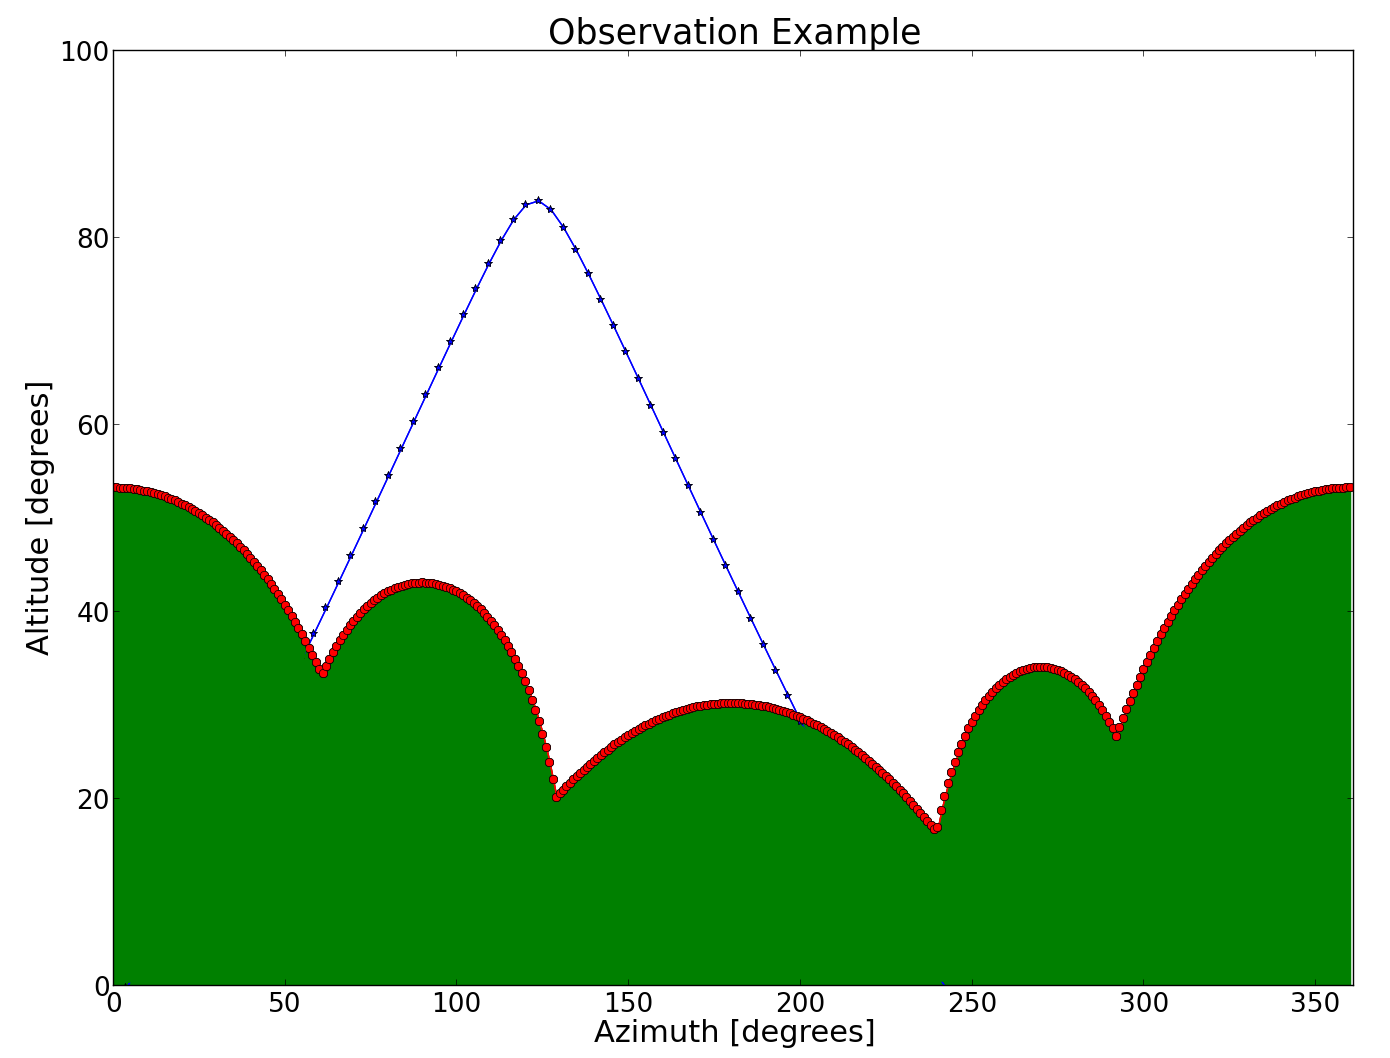
\includegraphics[scale=0.41]{mount.png}
\caption {An Example of a day of observation, where the red dots mark the limit due to some local obstacles
(at Leuschner Observatory) The star indicates the evolution of an aimed point in our grid in the course
of a day.} 
\label{mountain}
\end{figure}


\begin{figure}[H]
\center
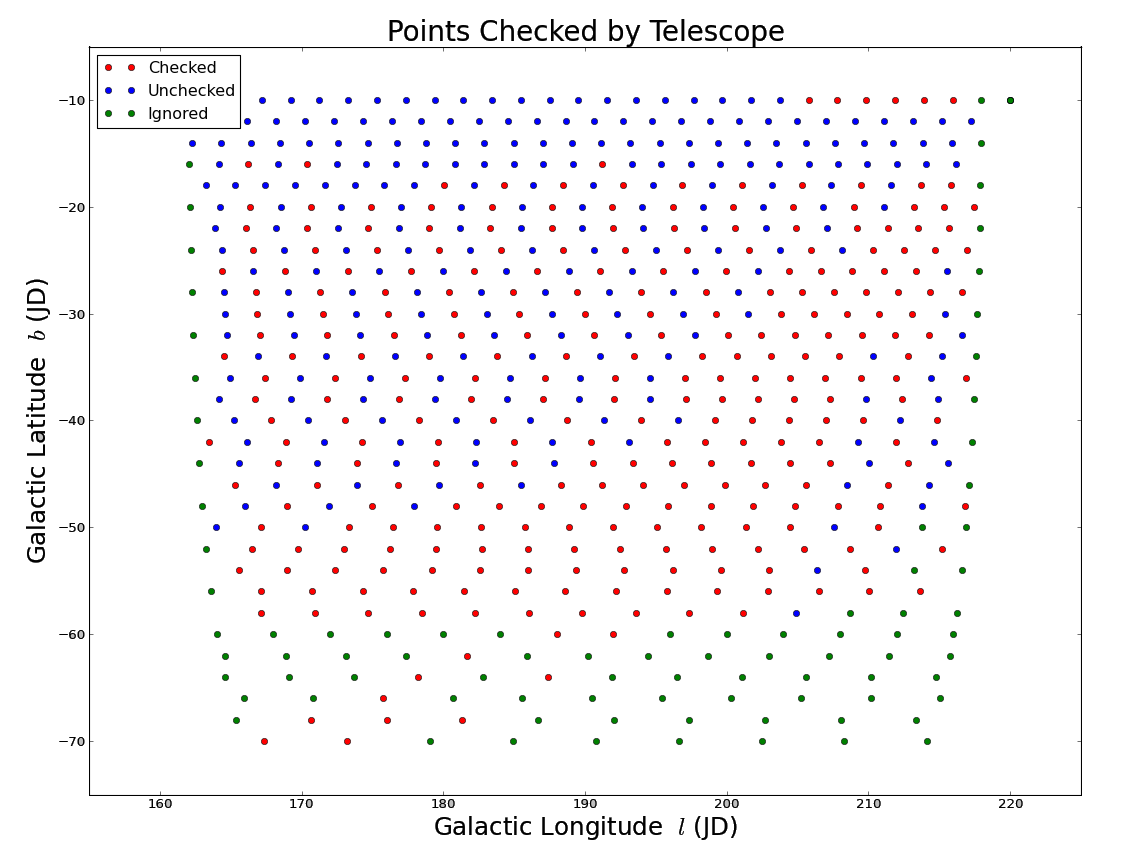
\includegraphics[scale=0.5]{grid.png}
\caption {A grid of the points checked in the sky as a result of our observations. The blue ones correspond
to the points we were about to check, but we didn't manage to collect the spectra of these positions. The
red ones we were able to collect, and the green ones we ignored in order to optmize the information about
the bubble collected in our observation time. As a result, our grid had around $400$ points about
the Orion-Eridanus Superbubble.} 
\label{Fig:1}
\end{figure}


\section{Controlling Leuschner}

The whole data aquisition was made by $Python$ scripts that tracked, set the telescope functions and
saved the data files. A telescope control code worked together with a rotation matrix function,
that changed the \emph{Galactic Coordinates} of our points into \emph{Horizontal Coordinates}, so that the
dish could track, since the telescope function inputs must be \emph{Altitude} and \emph{Azimuth}. The codes and
the math behind it was previously developed for the \emph{Interferometry Lab}, and the details for the
matrices contruction and how they were applied is well described by the article on the following link:
\href{https://github.com/leosattler/ugradio/tree/master/lab_interf}{git hub account, lab\_interf folder}. With the
need of a conversion from Galactic Coordinates, an aditional step was added, making use of the following
matrix provided by the casper website:

\begin{equation}
\mathbf{R}_{(\alpha,\delta)2000\rightarrow(l,b)} =
 \begin{bmatrix}
  -0.054876 & -0.873437 & -0.483835 \\
  0.494109  &  -0.444830 & -0.746982 \\  
  -0.867666 &  -0.198076 & 0.455984
 \end{bmatrix},
\end{equation}
which is a conversion for the \emph{epoch 2000}. The \emph{PyEphem} and 
\emph{radiolab} module were used to perform some calculations.

In fact the inverse of the previous matrix was used, and the following
matrix operations were applied to get the desired points in the sky:
\begin{equation}
\mathbf{R}_{(l, b) \rightarrow (az, alt)}=\mathbf{R}_{(ha, \delta) \rightarrow(az, alt)} \cdot \mathbf{R}_{(\alpha, \delta)\rightarrow (ha, \delta)} \cdot \mathbf{R}_{(l,b)\rightarrow(\alpha,\delta)}.
\label{eq:conv}
\end{equation}

For the antenna control, besides these modules, the following ones were used: 
\emph{dish}, \emph{dish\_synth} and \emph{takespec}. The first one was used to perform 
the movements of the telescope, as the tracking and homing, 
just turning the the noise diode of the telescope on and off, for purposes of measuring
the instrumentation noise for data calibration. Only one homing was necessary (in the beginning 
of each observation), and the tracking was made after finding the position in Altitude and
Azimuth, in degrees, for each point of interest. The second one was used to set some
values to the dish, as amplitude and frequency for the Local Oscsilator. The LO (Local Oscilator) frequency 
was $1272.4 \ MHz$, and the amplitude was $10 \ dBm$. The last module
takes the data and save in \emph{.log} files, later written with the module
\emph{readspec\_mod}. At the end of each pointing procedure, we ended up
with $4$ different files later used to perform the calibration, discussed in the next section.
All the codes for tracking and controlling the Leuschner dish can be found 
\href{https://github.com/leosattler/ugradio/tree/master/lab\_dish}{here}.

\section{Data Calibration}

In order to measure the column density by anylising the HI line profiles, we first treat the data
using the $4$ files created for each point. They were the \emph{Noise\_On}, \emph{Noise\_Off}, 
\emph{Spectra\_On} and \emph{Spectra\_Off}, meaning that we took $2$ spectra profiles: one 'On'
our target line, and another 'Off' by $-4 \ MHz$. Together with these $2$ spectra measurements,
we recorded a noise for both instances, hence \emph{Noise\_On} (recording the noise 'On' the
spectra) and \emph{Noise\_Off} (for the case we are off by $4 \ MHz$).

The math to calibrate the data is presented on the handout provided by the Radiolab instructors,
\emph{Calibrating the Intensity and Shape of Spectral Lines}, by Carl Heilies.
Severall steps were performed by using the so called \emph{cool method}. Basically, with all these
measurements, if we plot them on a same figure
we end up with $2$ distinct peaks, and they are off by the value set on the data aquisition 
for the LO ($4 \ MHz$), where the 'On' measurements are around the value of $1420.4 \ MHz$, as expected.
Besides them, we have $2$ spectra of the same profiles but with much higher intensity values. These are 
the noise values, used to calibrate the HI profile by correcting the instrument temperature. An example is shown in Fig.4. 

After the  corrections from the band pass
filter shape and all the added amplitude, related to the noise associated to our instruments,
we have a single featured emission line, which is the $21 \ cm$ line from the Orion-Eridanus
Superbubble region. One of its features is shown in Fig.5. As we know, many things can 
determine the shape of a spectral line. Basically, its position tells, at a 
first glence, about the elements
from the observed source. In our case we expect to see some line around $1420.4058 \ MHz$.
Its width reveals how hot the cloud is, just as the velocity range of the particles
from the cloud, due to Doppler effect. The Doppler effect can also 
give a lot of information  about the speed of the structure as, for example, if it 
rotates or expands. The shape of 
the peaks, and how far they are from the expected emission line (the one meassured at the
laboratory, for example), will tell about this.


\begin{figure}[H]
\center
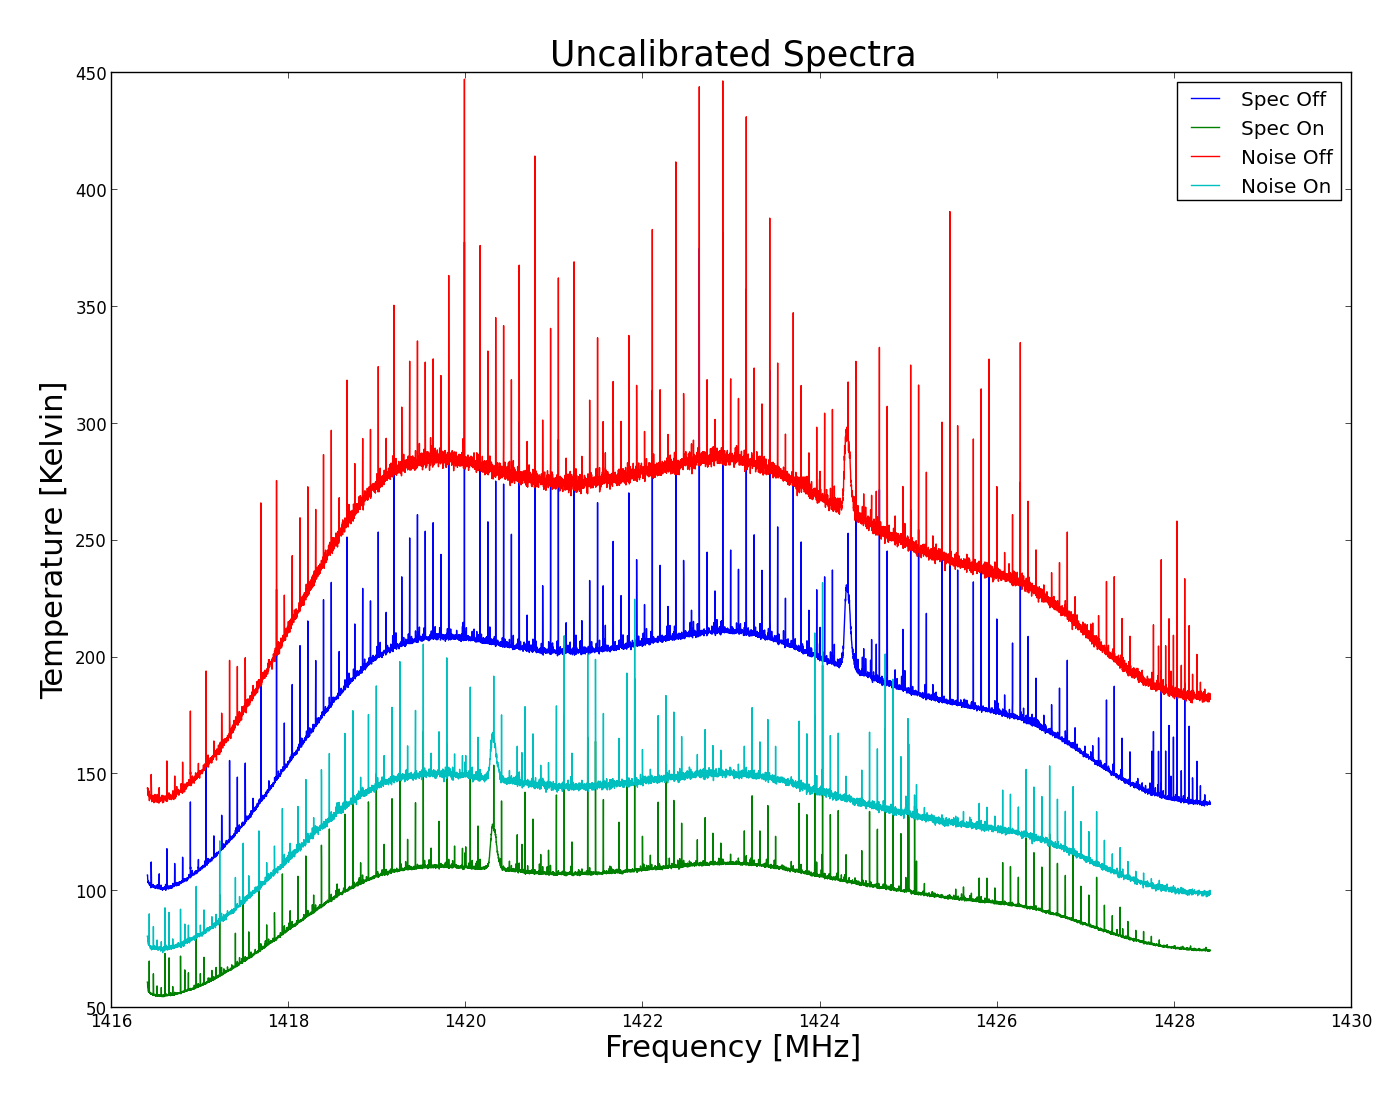
\includegraphics[scale=0.42]{uncal.png}
\caption {Figure showing the spectra for a point in the sky. These are the expected 
features for the observed points, presenting how our measurement looks like right
before proceeding through the calibration. The noise measurements, as outlined before, surpass
the \emph{Noise Off} spectra. The several peaks are detections from the
atmosphere and many other sources, due to the contamination of the city and other nearby emissions,for example. They are smoothed as a first calibration step.
Besides those, we see the four distinctive peaks corresponding to our
expected HI line emissions, that at this stage are dominated by all the noise present 
in our data.} 
\label{moon_win}
\end{figure}


As observed in Fig.5, the central peak is not quite at $1420.4 \ MHz$, which means that the bubble itself has a mean velocity related to us. Also, some features of peaks rising to the right and to the left of the central value are observed, revealing an expanding shell around the cavity of the
bubble, where the blueshifted spectra is an observation of material coming towards us, and 
the redshifted spectra is going away. In addition to that, we see a line with $2$ peaks,
which is propably the center of the expanding structure, showing both the approaching and
distancing features (redshift and blueshift) along our line of sight. And, finally,
a peak with no extra feature besides a single and narrow emission line, represents an
observation around the very edge of the bubble, where no Doppler shift is expected at all. 
 

\begin{figure}[H]
\center
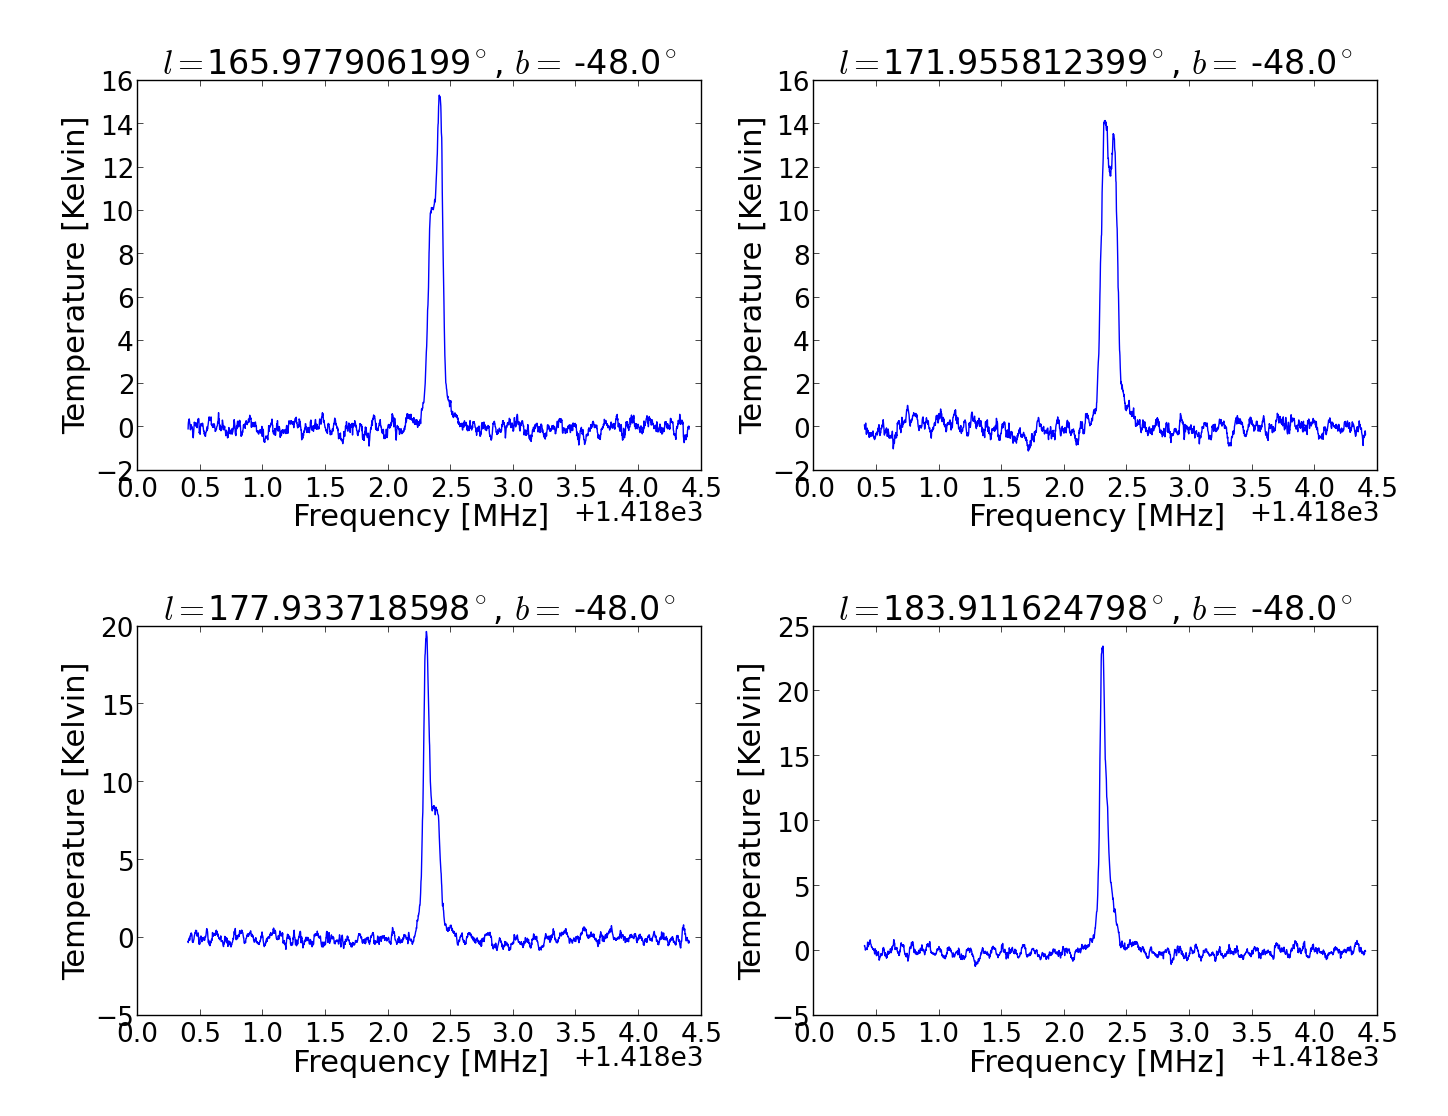
\includegraphics[scale=0.46]{calib.png}
\caption {Figure of $4$ calibrated spectra and its respective positions in the sky, 
in Galacti Coordinate (JD). These images show different features from the Orion-Eridanus
Superbubble with respect to the Doppler effect. These lines represent observations 
near the center (upper right), with $2$ shifted peaks, and on the very edge (bottom right),
with no Doppler shift. The ones on the left represent portions of the cloud that are either
expanding toward us (upper left) or going away from us (bottom left).} 
\label{moon_win}
\end{figure}


\section{Final Image} 

As a result, after all the points were calibrated, by using the equations from Section 2,
the final image of the Orion-Eridanus Superbubble is shown in the following pictures. The first one
is how actually we see the bubble structure in the sky, respecting the grid constructed by
the mapped points via Eq.3. We can compare with Fig.3 to in order to get a perception
of the sampled points and which features they represent in our final image. 

The second figure is a flat representation, with a rescaled grid to make a grid that 
can easilly show the position of each feature in the square grid. This is not actually
how we see the bubble in the sky, but can help to indentify the $l$ and $b$ in order
to work with this precise point, for purposes of reference or regions of interest, for example.

The construction of the images was made using a smoothing function, runing over a grid containing the integrated spectra of each point (resulting in a column density easurement via Eq.1). 
This smoothing was in fact a convolutioin with a $2D$ gaussian function, containing a spreading factor with the size of half the resolution of the main grid. The result of this convolution was devided by the result
of a second convolution, from the same gaussian function with a grid containing only $ones$, placed at the same index values corresponding to those containing values different from zero in the main grid.
This was done in order to normalize our first convolution, and the final 
result was more accurate in terms of how actually a point in the grid contributes for 
an intensity measurement.

\begin{figure}[H]
\center
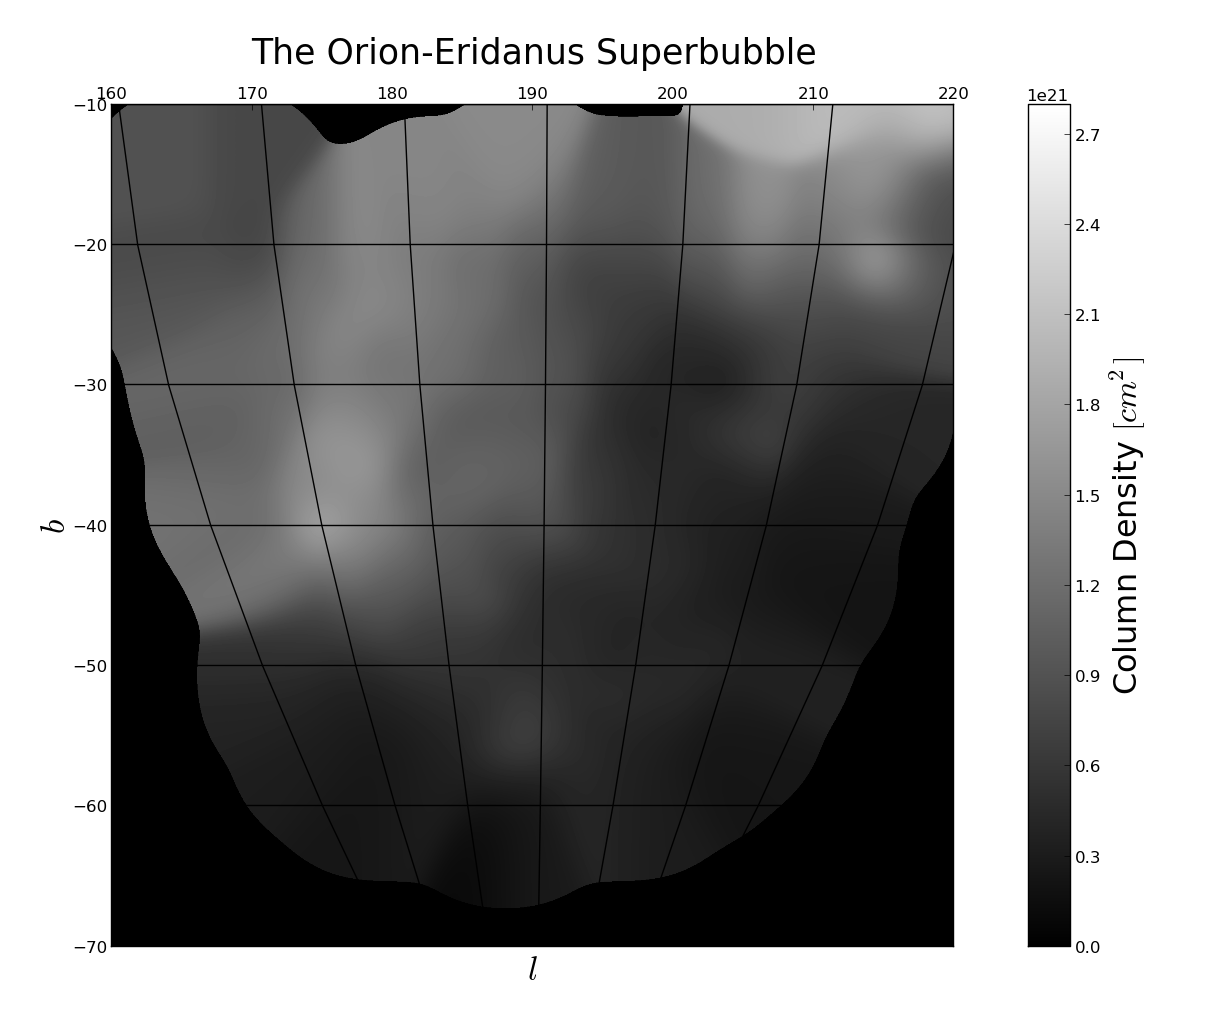
\includegraphics[scale=0.52]{final_orion_comprs.png}
\caption {The Orion-Eridanus Superbubble, real repesentation. 
This image was constructed with a 
$2000x2000$ grid by rescaling and replacing the points of the original grid
ilustrated by Fig.3. This main grid was than convolved and its convolution devided
by a normalizing array. Many of the features of an expanding shell can be seen,
just as a characteristic cavity surrounded by the cloud of Hydrogen. This thick
cloud is the main source of emisison of HI lines, leading to the emasurement of
the column density. We can observe that, in fact, in the center of the bubble there's a lack 
of material, what makes harder the detection of an expansion due to Doppler shift. The
dark areas around the image show the lack of point information in our constructed grid,
due to those that were neglected or those we could not achieve due to a limited time of
observation time. However, the main structure of the bubble can still be well observed.} 
\label{m17}
\end{figure}

\begin{figure}[H]
\center
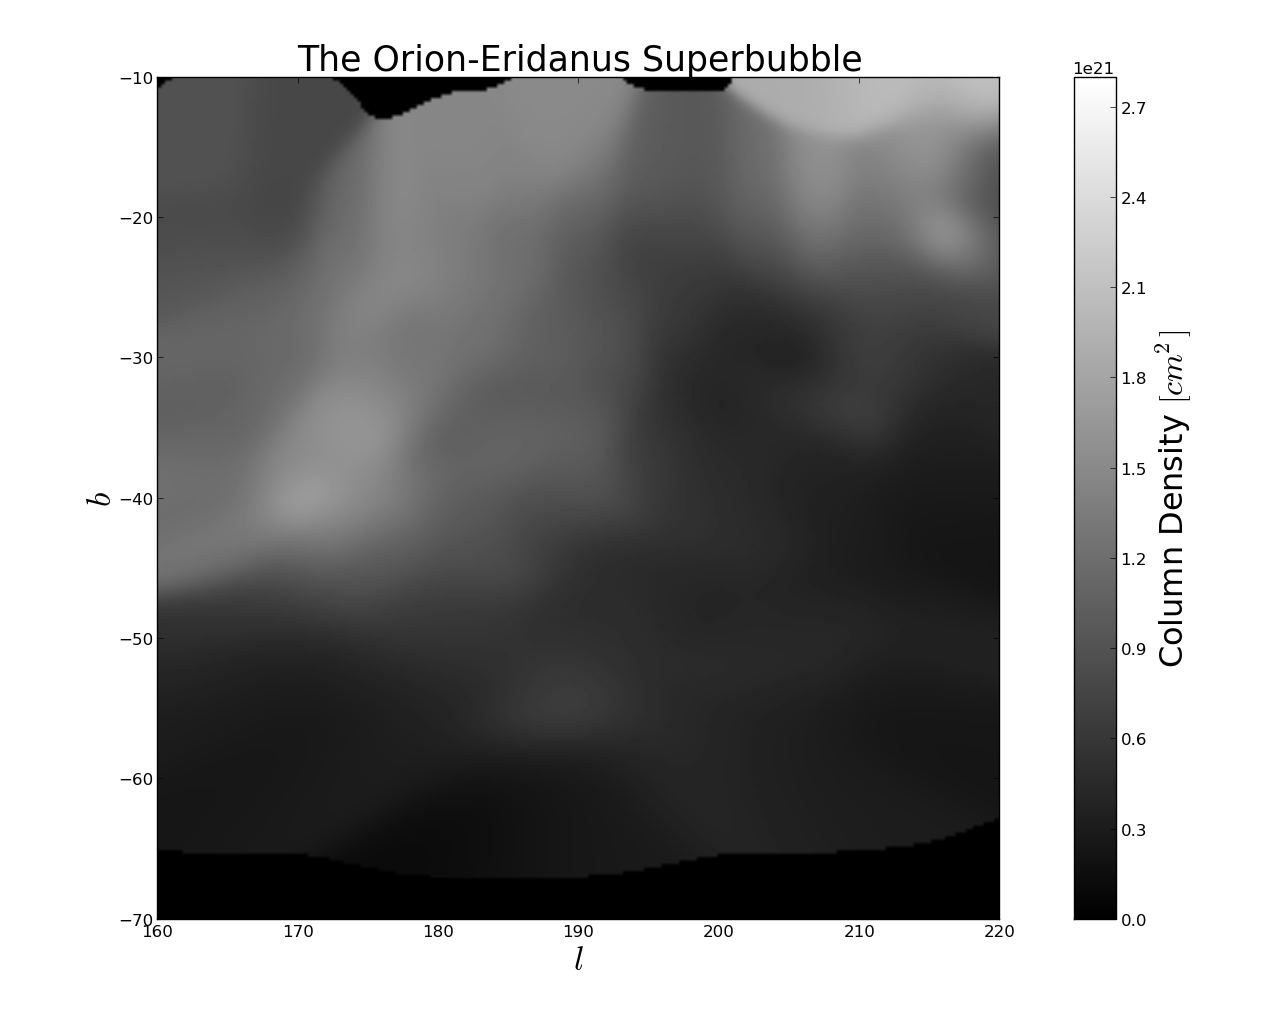
\includegraphics[scale=0.52]{final_orion_spred.png}
\caption {The Orion-Eridanus Superbubble, squared representation. 
This image was constructed with a 
$2000x2000$ grid by rescaling and replacing the points of the original grid
ilustrated by Fig.3. This main grid was than convolved and its convolution devided
by a normalizing array. At last, this grid was again rescaled to a square representation,
in order to have a different representation of the same structure. Also, this image
helps the comparisson with the next figure also containing the Orion-Eridanus Superbubble,
from A.G.A. Brown et. al. from the article \emph{The Orion OB1 association}, build with
data from the Galactic survey made with the $25 \ m$ Dwingeloo telescope, mapping the
$21 \ cm$ emission line with a $36'$ beam width. 
Many of the features of an expanding shell can be seen and compared,
just as a characteristic cavity surrounded by the cloud of Hydrogen. Again,
we see a large amount of gas in the upper part, also meaning that we did not loose 
much information from the bubble by neglecting those points below $l=-70^{circ}$.} 
\label{m17}
\end{figure}


\section{Conclusion}

In this lab, we were able to accuratly take and calibrate the measurement of 
intensity from a structure of Hydrogen, as shown by Fig. 5, where we can easilly 
observe the $21 \ cm$ emission line and the features related to the structure it came from. 
Also, it means that the rotation matrix developed to take the data, just as all the
telescope control scrpits, were well build and in deed work.
 
The measurement of Hydorgen column density, in order to create an image, and all the procedures
to finally create a grid with the information from all the points checked by the telescope,
can be compared with the follwing picture, from
A.G.A. Brown et. al. 1995, ApJ.:

\begin{figure}[H]
\center
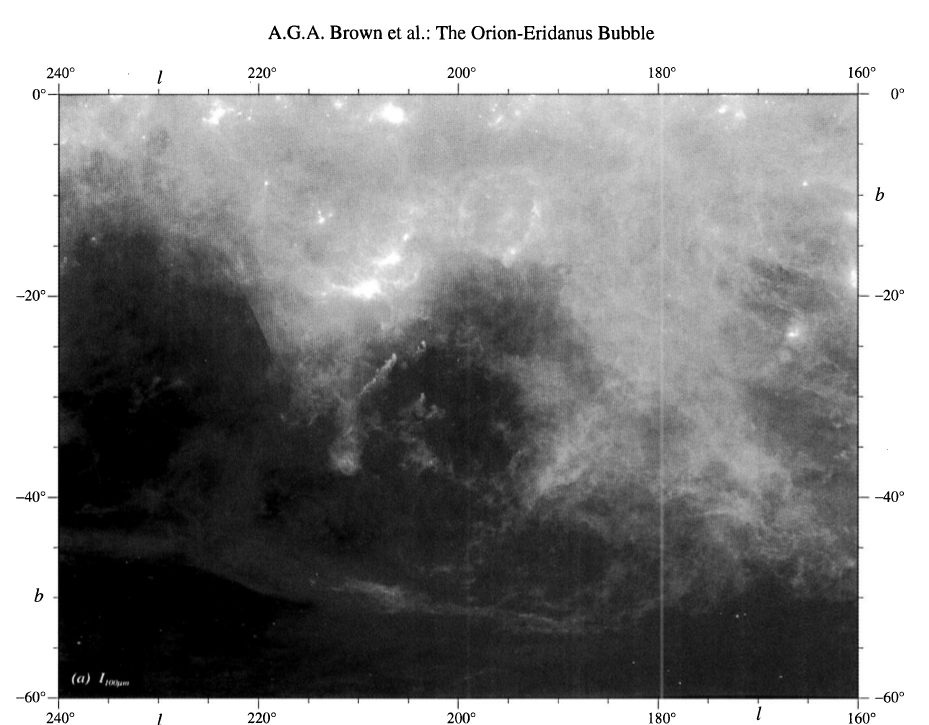
\includegraphics[scale=0.48]{article.png}
\caption {Image of the Orion-Eridanus Superbubble, build with
data from the Galactic survey made with the $25 \ m$ Dwingeloo telescope, mapping the
$21 \ cm$ emission line with a $36'$ beam width. The points in the sky are basically the same,
the only difference is that here the longitude axis range from $l=240^{circ}\rightarrow 160^{circ}$,
being flipped if compared to the same axis of Fig.7. The overall shape of
the bubble can be detected on both Fig.'s 6 and 7, by comparing them with this high resolution
image. This indicates that the whole process, from data aquisition, untill the 
construction of a final grid containig the calculated column density, 
was accuratly done, and despite our poor resolution
conditions, our image is correctly ilustrating the Orion-Eridanus Superbubble.} 
\label{moon_win}
\end{figure}

By comparing the last two images, knowing that their longitudinal 
axis grow in opposite directions, we are actually able to see the overall 
shape of a bubble and even the main features around its center. This basically 
shows that the procedure to get, treat and work with the data was well performed,
and altough we have a low resolution image, Fig.s 6 and 7 are acceptable 
representations of the Orion-Eridanus Superbubble.

Also, is a goal of the \emph{Daveandpals} group members to achieve a higher resolution by taking 
more data as soon as possible, and also exploring the Doppler information present in our data,
in order to evidenciate the parts of the bubble that are moving away from us
and approaching us and plot this feature. Also,
this could be  another option for measuring the density of material on the 
observed region of the sky. 

\end{document}


